\documentclass[10.5pt,a4paper]{article}
\usepackage[top=1.6cm,bottom=1.6cm,left=1.8cm,right=1.8cm]{geometry}
\usepackage[utf8]{inputenc}
\usepackage[T1]{fontenc}
\usepackage[french]{babel}
\usepackage{lmodern}
\usepackage{xcolor}
\usepackage{graphicx}
\usepackage{titlesec}
\usepackage{enumitem}
\usepackage{array}
\usepackage{tabularx}
\usepackage{booktabs}
\usepackage{hyperref}
\usepackage{fancyhdr}
\usepackage{lastpage}

\definecolor{agirhindigo}{HTML}{4F46E5}
\definecolor{agirhdark}{HTML}{1E1B4B}
\definecolor{agirhbg}{HTML}{EEF2FF}

\hypersetup{colorlinks=true,linkcolor=agirhindigo,urlcolor=agirhindigo,citecolor=agirhindigo}

\setlength{\parindent}{0pt}
\setlength{\parskip}{4pt}

\titleformat{\section}{\large\bfseries\color{agirhindigo}}{\thesection.}{0.5em}{}
\titlespacing*{\section}{0pt}{7pt}{3pt}

\setlist[itemize]{topsep=1pt,itemsep=1pt,parsep=0pt,leftmargin=1.3em}

\pagestyle{fancy}
\fancyhf{}
\renewcommand{\headrulewidth}{0.4pt}
\fancyhead[L]{\footnotesize\color{gray} arhia --- Synth\`ese des Travaux R\'ealis\'es (Soutenance PFA)}
\fancyhead[R]{\footnotesize\color{gray} Wilfried TSETSE --- ENSA Safi}
\fancyfoot[C]{\footnotesize\color{gray} \thepage/\pageref{LastPage}}

\newcommand{\code}[1]{\texttt{\small #1}}

\begin{document}

% ================= PAGE 1 : COUVERTURE =================
\thispagestyle{empty}
\begin{center}
  \vspace*{0.8cm}
  {\small \'Ecole Nationale des Sciences Appliqu\'ees de Safi}\\
  {\small Fili\`ere GIDIA --- Ann\'ee universitaire 2025--2026}

  \vspace{1.2cm}
  \raisebox{-0.5\height}{
\includegraphics[height=1.4cm]{ensa-logo.png}}\hspace{1.3cm}\raisebox{-0.5\height}{
\includegraphics[height=1.4cm]{agirh-logo.png}}

  \vspace{1cm}
  {\normalsize\bfseries\color{agirhdark} SYNTH\`ESE DES TRAVAUX R\'EALIS\'ES}\\[2pt]
  {\small\itshape Support de questions --- Soutenance de Projet de Fin d'Ann\'ee (PFA)}

  \vspace{0.8cm}
  {\Huge\bfseries\color{agirhindigo} arhia}\\[3pt]
  {\small\itshape\color{agirhdark} (Agent RH IA)}\\[5pt]
  {\Large\color{agirhdark} Assistant RH agentique pour l'Onboarding et l'Offboarding}

  \vspace{0.5cm}
  \textcolor{agirhindigo}{\rule{0.5\textwidth}{0.8pt}}

  \vspace{0.5cm}
  {\large\itshape R\'epondre aux questions RH (RAG document\'e) et informer sur l'avancement\\ d'un dossier --- sans jamais ex\'ecuter d'action irr\'eversible depuis la conversation.}

  \vspace{0.9cm}
  {\small
    \begin{tabularx}{0.8\textwidth}{@{}X X@{}}
      \toprule
      \textbf{R\'ealis\'e par} & \textbf{Encadrant} \\
      \midrule
      M. Komla Edem Wilfried Tsetse & M. Moulay Rachid Didi Alaoui \\
      \bottomrule
    \end{tabularx}
  }

  \vspace{0.35cm}
  {\small D\'ep\^ot GitHub priv\'e, accessible sur demande : \href{https://github.com/wekt2k04/arhia}{github.com/wekt2k04/arhia}}

  \vspace{1.3cm}
  {\small
    \begin{tabular}{@{}l l@{}}
      \textbf{1.} Contexte et strat\'egie & p.~2 \\
      \textbf{2.} Architecture et stack technique & p.~2 \\
      \textbf{3.} C\oe{}ur du projet : sous-syst\`eme IA & p.~3 \\
      \textbf{4.} Workflows m\'etier & p.~3 \\
      \textbf{5.} Bilan v\'erifi\'e + tableau r\'ecapitulatif & p.~3 \\
    \end{tabular}
  }
\end{center}

\newpage

% ================= PAGE 2 =================
% ---------- 1. Contexte ----------
\section{Contexte et strat\'egie}
\begin{itemize}
  \item Agent conversationnel d\'edi\'e \`a l'onboarding et \`a l'offboarding : politiques RH (RAG document\'e) + suivi de dossier.
  \item Contrainte de conception assum\'ee : \textbf{jamais} d'action irr\'eversible d\'eclench\'ee depuis la conversation.
  \item Une premi\`ere it\'eration a \'et\'e r\'e-audit\'ee en cours de stage et recentr\'ee strictement sur l'onboarding/offboarding --- \textbf{cette fiche d\'ecrit l'\'etat actuel, fonctionnel de bout en bout.}
\end{itemize}

% ---------- 2. Architecture ----------
\section{Architecture et stack technique}
\begin{itemize}
  \item \textbf{.NET 8}, architecture \textbf{hexagonale} \`a 4 couches : Domain $\rightarrow$ Core $\rightarrow$ Infrastructure $\rightarrow$ Api (une couche ne d\'epend que de celles list\'ees en dessous).
  \item Frontend \textbf{Next.js 15} en \textbf{BFF} --- le JWT n'est jamais expos\'e au navigateur (cookie \code{httpOnly}).
  \item \textbf{Auth \& RBAC} : JWT + Identity, 3 r\^oles (\code{Employee}/\code{HR}/\code{QualityAdmin}), port\'ee d\'epartement v\'erifi\'ee \emph{avant} le r\^ole.
  \item Donn\'ees : \textbf{SQL Server} (m\'etier) + \textbf{Qdrant} (index vectoriel RAG). Temps r\'eel : \textbf{SSE} (chat + notifications).
  \item D\'eploiement : \textbf{Docker Compose} (4 services) + Ollama natif sur l'h\^ote.
\end{itemize}

\vspace{2pt}
\begin{center}
  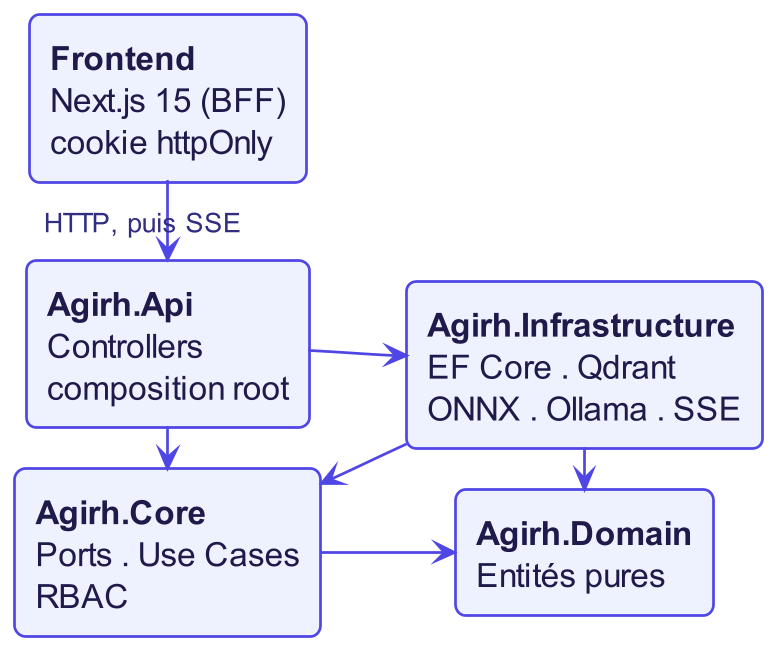
\includegraphics[width=0.62\textwidth]{architecture.png}
\end{center}

\newpage

% ================= PAGE 3 =================
% ---------- 3. IA ----------
\section{C\oe{}ur du projet : sous-syst\`eme IA}
\begin{itemize}
  \item Pipeline \textbf{RAG en 4 phases obligatoires} : chunking structurel $\rightarrow$ embedding ONNX (768d) $\rightarrow$ stockage \textbf{Qdrant} (ANN/HNSW) $\rightarrow$ \textbf{reranking} cross-encodeur.
  \item \textbf{Router} (Ollama, \code{phi4-mini:3.8b}) classe l'intention ; sortie jamais utilis\'ee telle quelle --- retombe sur \emph{hors p\'erim\`etre} par d\'efaut (\textbf{fail-safe, pas fail-open}).
  \item Le point le plus important du projet : \textbf{2 portes de sortie anticip\'ee, en code}, avant tout appel au Generator --- garde-fou anti-hallucination v\'erifiable et test\'e, pas une simple consigne de prompt.
  \item \textit{Limite mesur\'ee et assum\'ee} : $\sim$27\% d'erreur de routage sur un jeu de 48 questions test, avec le mod\`ele actuel sur mat\'eriel local sans GPU --- document\'ee plut\^ot que masqu\'ee, sans impact sur le garde-fou (plan de d\'eport de charge en \S5).
\end{itemize}

\vspace{4pt}
\begin{center}
  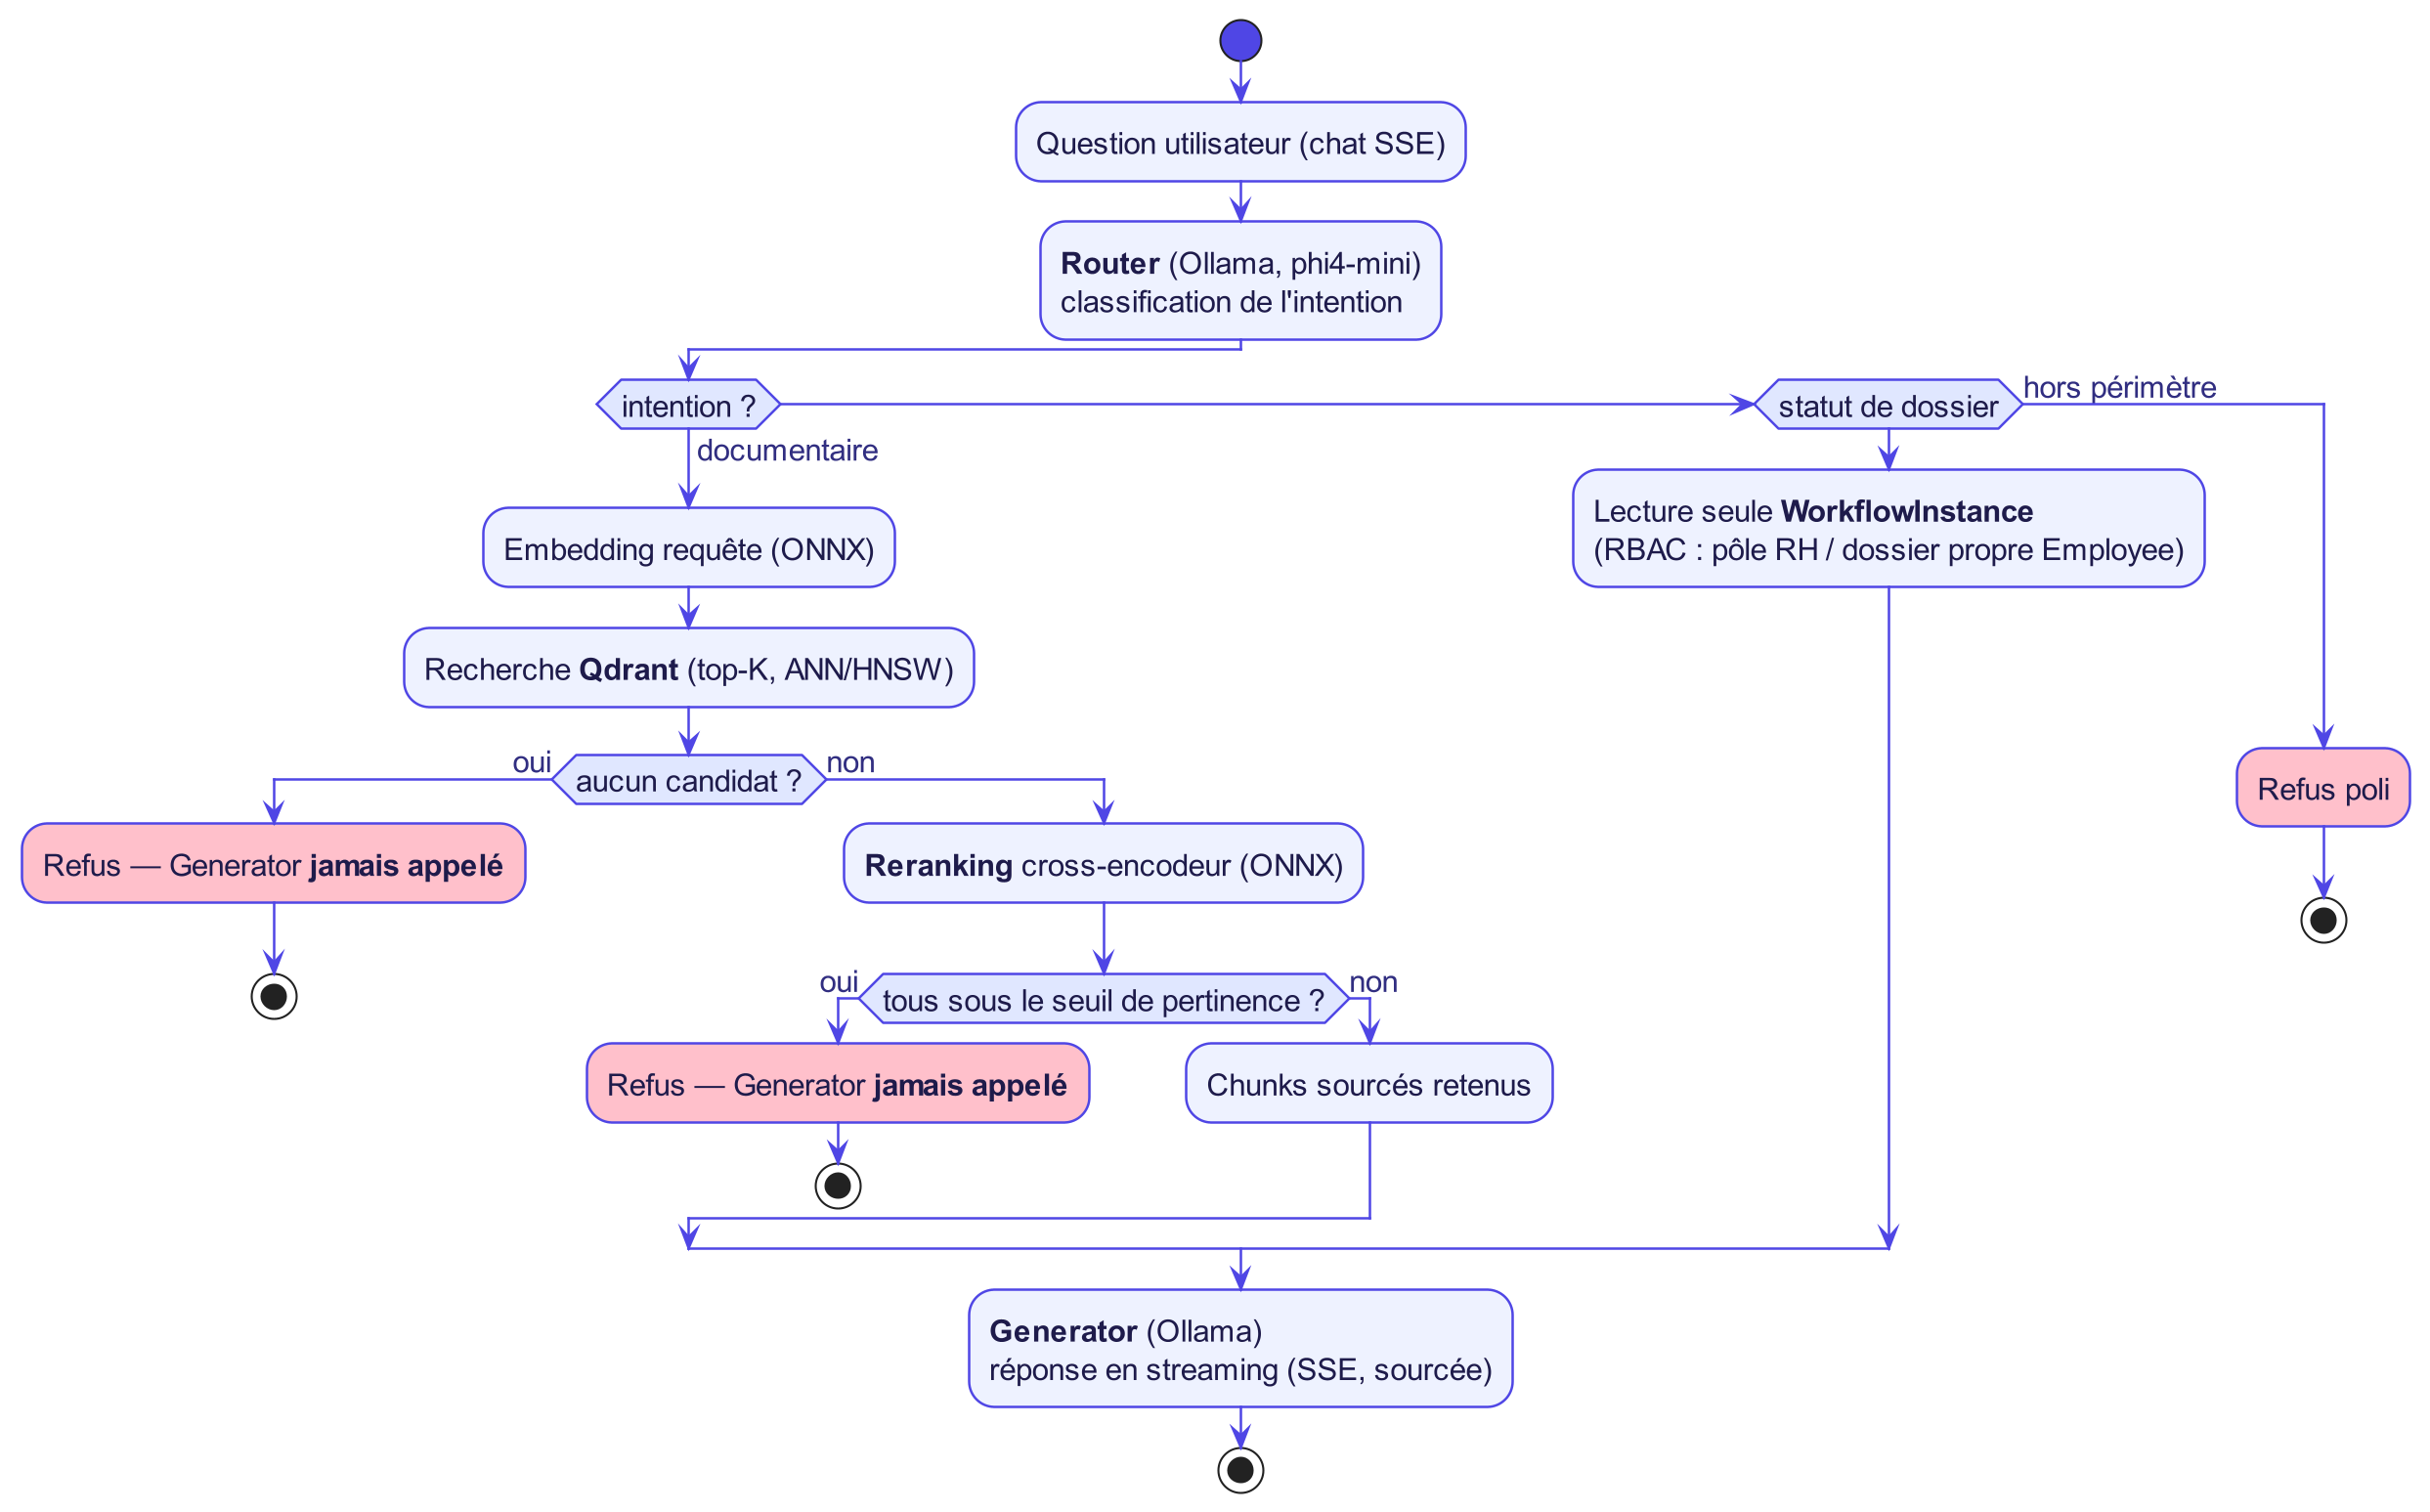
\includegraphics[width=0.55\textwidth]{ai_pipeline.png}
\end{center}

% ---------- 4. Workflows ----------
\section{Workflows m\'etier}
\begin{itemize}
  \item \textbf{Onboarding} : fiche collaborateur $\rightarrow$ items r\'esolus (Poste $\times$ D\'epartement $\times$ Contrat) contre le template approuv\'e $\rightarrow$ checklist persist\'ee $\rightarrow$ cl\^oture $\rightarrow$ archivage lecture seule.
  \item \textbf{Offboarding} : m\^eme m\'ecanique g\'en\'erique (aucune distinction de code) --- checklist d\'edi\'ee d\'eriv\'ee d'un document r\'eel (\code{SMSI.ENR.10-2}).
  \item \textbf{Circuit qualit\'e des templates} : R\'edacteur propose $\rightarrow$ V\'erificateur $\rightarrow$ Approbateur --- seul un template \emph{Approved} peut instancier un dossier r\'eel, contrainte v\'erifi\'ee par le code.
\end{itemize}

\vspace{2pt}
\begin{center}
  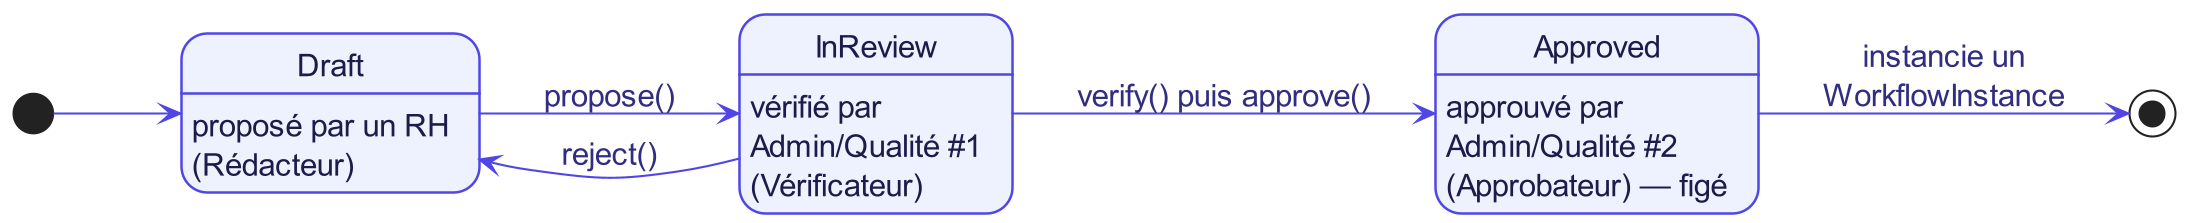
\includegraphics[width=0.68\textwidth]{workflow_circuit.png}
\end{center}

% ---------- 5. Bilan ----------
\section{Bilan v\'erifi\'e}
\begin{itemize}
  \item \textbf{211 tests automatis\'es} (xUnit/Moq/FluentAssertions), \textbf{0 warning} au build. Pipeline RAG et chat v\'erifi\'es en HTTP r\'eel de bout en bout (streaming inclus).
  \item D\'eploiement Docker Compose v\'erifi\'e sur base fra\^iche : inscription $\rightarrow$ connexion $\rightarrow$ chat sourc\'e.
  \item \textit{Suite pr\'evue} : d\`es le \textbf{jeudi 27 ao\^ut 2026} (retour en entreprise), d\'eporter Router et Generator vers le \textbf{serveur Ollama de l'entreprise} (\code{192.168.100.220:11434}) --- \code{phi4:14b} (m\^eme famille que le mod\`ele actuel) \`a l'essai pour le Router, \code{gemma4:12b} (d\'ej\`a identifi\'e comme candidat mais \'ecart\'e en local faute de GPU) pour le Generator --- puis endpoints de lecture/liste, trois cas particuliers m\'etier encore ouverts.
\end{itemize}

\vspace{3pt}
\begin{center}\small
\begin{tabularx}{\textwidth}{@{}l X@{}}
\toprule
\textbf{Composant} & \textbf{\'Etat} \\
\midrule
Architecture & Hexagonale, 4 couches --- op\'erationnelle \\
Backend / Frontend & .NET 8 / Next.js 15 (BFF) --- 211 tests verts, 0 warning \\
S\'ecurit\'e & JWT + RBAC (3 r\^oles) + port\'ee d\'epartement v\'erifi\'ee \\
RAG & 4 phases (chunking / embedding / Qdrant / reranking) --- v\'erifi\'e en HTTP r\'eel \\
Garde-fou anti-hallucination & 2 portes de sortie anticip\'ee en code --- test\'e \\
Router & Classification 3 intentions --- $\sim$27\% d'erreur (mat\'eriel local, isol\'ee) ; d\'eport serveur entreprise pr\'evu 27/08 \\
Workflows & Onboarding + Offboarding, m\'ecanique g\'en\'erique --- op\'erationnels de bout en bout \\
D\'eploiement & Docker Compose (4 services) + Ollama natif --- v\'erifi\'e sur base fra\^iche \\
\bottomrule
\end{tabularx}
\end{center}

\end{document}
